\documentclass{article}
\usepackage[english]{babel}
\usepackage{amssymb,graphicx,bbm,latexsym}

%%%%%%%%%% Start TeXmacs macros
\catcode`\<=\active \def<{
\fontencoding{T1}\selectfont\symbol{60}\fontencoding{\encodingdefault}}
\catcode`\>=\active \def>{
\fontencoding{T1}\selectfont\symbol{62}\fontencoding{\encodingdefault}}
\newcommand{\nobracket}{}
\newcommand{\tmop}[1]{\ensuremath{\operatorname{#1}}}
\newcommand{\tmtextit}[1]{{\itshape{#1}}}
\newcommand{\tmverbatim}[1]{{\ttfamily{#1}}}
\newenvironment{proof}{\noindent\textbf{Proof\ }}{\hspace*{\fill}$\Box$\medskip}
\newtheorem{conjecture}{Conjecture}
\newtheorem{corollary}{Corollary}
\newtheorem{definition}{Definition}
\newtheorem{lemma}{Lemma}
\newtheorem{proposition}{Proposition}
\newtheorem{theorem}{Theorem}
%%%%%%%%%% End TeXmacs macros

\begin{document}

\title{An Expression For The Argument of $\zeta$ at Zeros on the Critical
Line}

\author{Stephen Crowley <stephencrowley214@gmail.com>}

\maketitle

\begin{abstract}
  It is conjectured that when $t = t_n$ is the imaginary part of the $n$-th
  zero of $\zeta$ on the critical line, the normalised argument $S (t_{})_{} =
  \pi^{- 1} \arg \zeta \left( \frac{1}{2} + i t_{} \right)$ is equal to $S (t)
  = S_n (t_n) =_{} n - \frac{3}{2} - \frac{\vartheta (t_n)}{\pi}$ where \
  $\vartheta (t)$ is the Riemann-Siegel $\vartheta$ function. If $S (t_n) =
  S_n (t_n) \forall n \in \mathbbm{Z}^+$ then the exact transcendental
  equation for the Riemann zeros has a solution for each positive integer $n$
  which proves that Riemann's hypothesis is true since the counting function
  for zeros on the critical line is equal to the counting function for zeros
  on the critical strip in that case.
\end{abstract}

\section{Introduction}

\subsection{Motivation}

The goal of this paper is to show that a solution $t_n$ exists for each $n$ of
the exact transcendental equation for the Riemann zeros

\begin{definition}
  The \tmverbatim{exact equation} for the imaginary part of the $n$-th zero of
  $\zeta$ on the critical line
  \begin{equation}
    \frac{\vartheta (t_n)}{\pi} + S (t_n) + 1 = n - \frac{3}{8}
  \end{equation}
\end{definition}

which is the same equation as in {\cite[Equation 20]{z0t}} but with 1 added to
both the left and right sides of the equation. $\zeta \left( \frac{1}{2} + i
t_n \right) = 0$

\

\subsubsection{The Riemann-Siegel $\vartheta (t)$ Function}

The Riemann-Siegel $\vartheta$ function is defined by
\begin{equation}
  \begin{array}{cl}
    \vartheta (t) & = - \frac{i}{2} \left( \ln \Gamma \left( \frac{1}{4} +
    \frac{i t}{2} \right) - \ln \Gamma \left( \frac{1}{4} - \frac{i t}{2}
    \right) \right) - \frac{\ln (\pi) t}{2} \text{}\\
    & = \arg \left( \Gamma \left( \frac{1}{4} + \frac{i t}{2} \right) \right)
    - \frac{\ln (\pi) t}{2}
  \end{array}
\end{equation}
Let
\[ \tilde{\vartheta} (t) = \frac{t \ln \left( \frac{t}{2 \pi e} \right)}{2} -
   \frac{\pi}{8} \]
be the approximate $\vartheta$ function where the $\Gamma$ function has been
replaced with its Stirling approximation.
\begin{equation}
  \Gamma (s) \simeq \sqrt{2 \pi} s^{s - \frac{1}{2}} e^{- s}
\end{equation}
The $\vartheta (t)$ function is not invertible but the inverse of its
approximation $\tilde{\vartheta} (t)$ is defined by a linear function of the
Lambert W function given by
\begin{equation}
  \tilde{\vartheta}^{- 1} (t) = \frac{\pi + 8 t}{4 W \left( \frac{\pi + 8 t}{8
  \pi e} \right)}
\end{equation}
Let $\tmop{frac} (x) = \left\{ \begin{array}{ll}
  x - \lfloor x \rfloor & x \geqslant 0\\
  x - \lceil x \rceil & x < 0
\end{array} \right. \forall x \in \mathbbm{R}$ be the function which gives the
fractional part of a real number by subtracting either the floor $\lfloor x
\rfloor$ or the ceiling $\lceil x \rceil$ of $x$ from $x$, depending upon its
sign. Furthermore, let
\begin{equation}
  S (t) = \pi^{- 1} \arg \left( \zeta \left( \frac{1}{2} + \tmop{it} \right)
  \right) = \lim_{\varepsilon \rightarrow 0}  \frac{1}{2} ((S \nobracket (t +
  i \varepsilon) - S (t - i \varepsilon))
\end{equation}
be the argument of $\zeta$ on the critical line.

\begin{definition}
  The Riemann-von-Mangoldt formula makes use of Cauchy's argument principle to
  count the number of zeros \tmverbatim{inside the critical strip} $0 <
  \tmop{Im} (\rho_n) < t$ where $\zeta (\sigma + i \rho_n)$ with $0 < \sigma <
  1$
  \begin{equation}
    \tilde{N}_s (t) = \frac{t}{2 \pi} \ln \left( \frac{t}{2 \pi e} \right) +
    \frac{7}{8} + S (t) + O (t^{- 1})
  \end{equation}
  and this definition does not depend on the Riemann hypothesis(Conjecture
  \ref{RH}). This equation has exactly the same form as the asymptotic
  Equation \ref{ae}. {\cite[Equation 15]{z0t}}
\end{definition}

\begin{definition}
  The \tmverbatim{asymptotic equation} for the $n$-th zero of the Hardy $Z$
  function
  \begin{equation}
    \frac{t_n}{2 \pi} \ln \left( \frac{t_n}{2 \pi} \right) + S (t_n) + O
    \left( \frac{1}{t_n} \right) + 1 = n - \frac{3}{8} \label{ae}
  \end{equation}
  {\cite[Equation 20]{z0t}}
\end{definition}

\begin{corollary}
  The number of solutions of the asymptotic equation (\ref{ae}) for the zeros
  of the Hardy $Z (t)$ function, over the interval $[0, t]$ is given by
  \begin{equation}
    \tilde{N}_l (t) = \frac{t}{2 \pi} \ln \left( \frac{t}{2 \pi e} \right) +
    \frac{7}{8} + S (t) + O (t^{- 1}) \label{N0}
  \end{equation}
\end{corollary}

which counts the number of zeros \tmverbatim{on the critical line}.

\

\begin{conjecture}
  \label{ec}The \tmverbatim{exact equation} for the imaginary part of the
  $n$-th zero of $\zeta \left( \frac{1}{2} + i t \right)${\cite[Equation
  20]{z0t}}
  \begin{equation}
    \begin{array}{cc}
      \frac{\vartheta (t_n)}{\pi} + S (t_n) - \left( n - \frac{3}{2} \right)
      \pi & = 0 = \frac{\vartheta (t_n)}{\pi} + \frac{\arg \left( \zeta \left(
      \frac{1}{2} + \tmop{it} \right) \right)}{\pi} - \left( n - \frac{3}{2}
      \right) \pi
    \end{array} \label{ee}
  \end{equation}
  has a solution for each integer $n \geqslant 1$ where $t_n$ enumerate the
  zeros of $Z$ on the real line and the zeros of $\zeta$ on the critical line
  \begin{equation}
    \zeta \left( \frac{1}{2} + i t_n \right) = 0 \forall n \in \mathbbm{Z}^+
  \end{equation}
  where $\mathbbm{Z}^+$ denotes the positive integers. {\cite[Equation
  14]{z0t}}
\end{conjecture}

\subsection{The Gram Points}

The $n$-th Gram point is defined to be the solution of the equation
\begin{equation}
  \vartheta (t) = (n - 1) \pi
\end{equation}
A very accurate approximation $\tilde{g} (n)$ to the Gram points is $g (n)$ is
found by inverting $\tilde{\vartheta} (t)$ to get the exact solution
\begin{equation}
  \begin{array}{cl}
    \tilde{g} (n) & = \{ t : \tilde{\vartheta} (t) - (n - 1) \pi = 0 \}\\
    & = \left\{ t : \left( \frac{t \ln \left( \frac{t}{2 \pi e} \right)}{2} -
    \frac{\pi}{8} \right) - (n - 1) \pi = 0 \right\}\\
    & = \frac{(8 n - 7) \pi}{4 W \left( \frac{8 n - 7}{8 e} \right)}\\
    & = g (n) + O (\delta_n)
  \end{array}
\end{equation}
where $W$ is the Lambert W function, and the approximation bounds $\delta_n$
when $n = 1$ is $\delta_1 = 0.00223698 \ldots$, followed by $\delta_2 =
0.00137812 \ldots$ and decreases monotonically with increasing $n$, that is,
$\delta_{n + 1} < \delta_n$. \ The inverse of $\tilde{g} (n)$ is given by
\begin{equation}
  \begin{array}{ll}
    \tilde{g}^{- 1} (n) & = \{ t : \tilde{g} (n) = 0 \}\\
    & = \frac{t \ln \left( \frac{t}{2 \pi e} \right)}{2 \pi} + \frac{7}{8}\\
    & = \tilde{N} (t) - S (t)\\
    & = \tilde{N} (t) - S (t)
  \end{array}
\end{equation}
where $\tilde{N} (t)$=$\tilde{N}_s (t) = \tilde{N}_l (t)$.

\subsubsection{An Expression for $S (t)$ at its Discontinuous Points}

Define the infinite sequence of functions indexed by $n \in \mathbbm{Z}^+$
\begin{equation}
  \begin{array}{cl}
    T_n (t) & = 1 + \lfloor \tilde{g}^{- 1} (n) \rfloor - n\\
    & = 1 + \lfloor \frac{t \ln \left( \frac{t}{2 \pi e} \right)}{2 \pi} +
    \frac{7}{8} \rfloor - n
  \end{array}
\end{equation}
\begin{proposition}
  For each ``bad'' Gram point $n$ there will be, within $n \pm 2$, a
  corresponding zero on the critical line which has an argument not on the
  principal branch. That is, if $n$ is a ``bad'' Gram point then $T_m (t_m)
  \neq 0$ for some $m$ where $| m - n | \leqslant 2$.
\end{proposition}

The function $T_n = T_n (t_n)$ determines how many multiples of $\pi$ to add
or subtract to $- \frac{1}{2} - \lfloor \frac{\vartheta (t_n)}{\pi} \rfloor$
so that it agrees with the argument of $\zeta$ at a zero on the critical line
where it is discontinuous, jumping by the multiplicity of the corresponding
root, and having the value $\left. \lim_{\varepsilon \rightarrow 0} 
\frac{1}{2} ((S (\rho + i \varepsilon) - S (\rho - i \varepsilon) \right)$
when $\zeta (\rho) = 0$.

\begin{definition}
  Let
  \begin{equation}
    \begin{array}{ll}
      S_n (t_{}) & = \frac{1}{2} - \tmop{frac} \left( \frac{\vartheta
      (t)}{\pi} \right) - T_n (t)\\
      & = \frac{1}{2} - \tmop{frac} \left( \frac{\vartheta (t)}{\pi} \right)
      - (1 + \lfloor \tilde{g}^{- 1} (n) \rfloor - n)\\
      & =_{} \frac{1}{2} - \tmop{frac} \left( \frac{\vartheta (t)}{\pi}
      \right) - 1 - \lfloor \tilde{g}^{- 1} (n) \rfloor + n\\
      & =_{} - \frac{1}{2} - \tmop{frac} \left( \frac{\vartheta (t)}{\pi}
      \right) - \lfloor \tilde{g}^{- 1} (n) \rfloor + n\\
      & = n_{} - \frac{1}{2} - \tmop{frac} \left( \frac{\vartheta (t)}{\pi}
      \right) - \lfloor \tilde{g}^{- 1} (n) \rfloor\\
      & =_{} n - \frac{1}{2} - \tmop{frac} \left( \frac{\vartheta (t)}{\pi}
      \right) + \lfloor \frac{\vartheta (t)}{\pi} + 1 \rfloor\\
      & = n - \frac{1}{2} - \left( \frac{\vartheta (t)}{\pi} + 1 \right)\\
      & = n - \frac{1}{2} - \frac{\vartheta (t)}{\pi} - 1\\
      & = n - \frac{3}{2} - \frac{\vartheta (t)}{\pi}
    \end{array}
  \end{equation}
\end{definition}

Where we see that
\begin{equation}
  S_n (t_n) = n - \frac{3}{2} - \frac{\vartheta (t_n)}{\pi} = S (t_n)
\end{equation}
when $t_n$ is the imaginary part of a zero of $\zeta$ on the critical line.

\begin{conjecture}
  \label{c}The normalized argument $S (t) = \pi^{- 1} \arg \zeta \left(
  \frac{1}{2} + i t \right)$ at the n-th non-trivial zero \ $\zeta \left(
  \frac{1}{2} + i t_n \right) = 0 \forall n \geqslant 1$ on the critical line
  is equal to $S_n (t)$, that is
  \begin{equation}
    \begin{array}{cl}
      S (t_n) & = S_n (t_n) = \frac{1}{2} (\lim_{t \rightarrow t^-_n} S (t_{})
      + \lim_{t \rightarrow t^+_n} S (t_{}))\\
      & = n - \frac{3}{2} - \frac{\vartheta (t_n)}{\pi}
    \end{array} \label{een}
  \end{equation}
\end{conjecture}

\begin{theorem}
  If Conjecture \ref{c} is true then Conjecture \ref{ec} is true and, due to
  $\tmop{Lemma}$ \ref{fl}, so is Conjecture \ref{RH}, the Riemann hypothesis.
\end{theorem}

\begin{proof}
  If $s_{\vartheta} (t) S_n (t_n)$=$S (t_n)$ then $S (t_n)$ is well-defined
  $\forall n \geqslant 1$ since $s_{\vartheta} (t) S_n (t_n)$ is well-defined
  $\forall n \geqslant 1$.
\end{proof}

\begin{figure}[h]
  \resizebox{5.5in}{2.5in}{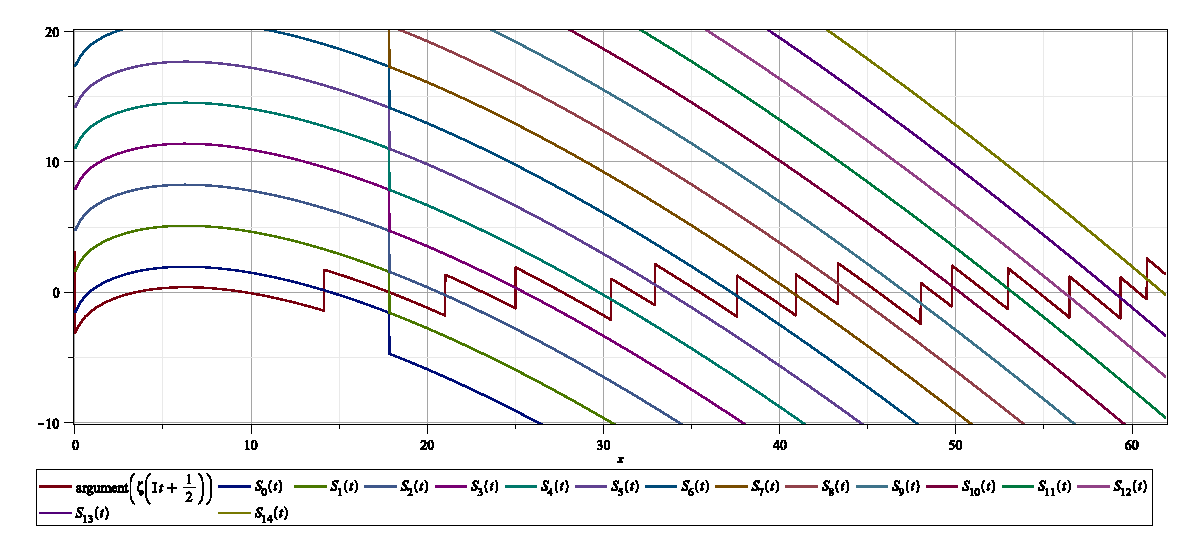
\includegraphics{liftedTwisted.eps}}
  \caption{$S_n (t)$ and the imaginary parts of the roots of $\zeta \left(
  \frac{1}{2} + i t_n \right)$ marked with verticle lines just touching its
  touching its corresponding pair of neighboring curves $S_n (t)$ for $n = 0
  \ldots 14$}
\end{figure}

\begin{figure}[h]
  \resizebox{5.5in}{2.5in}{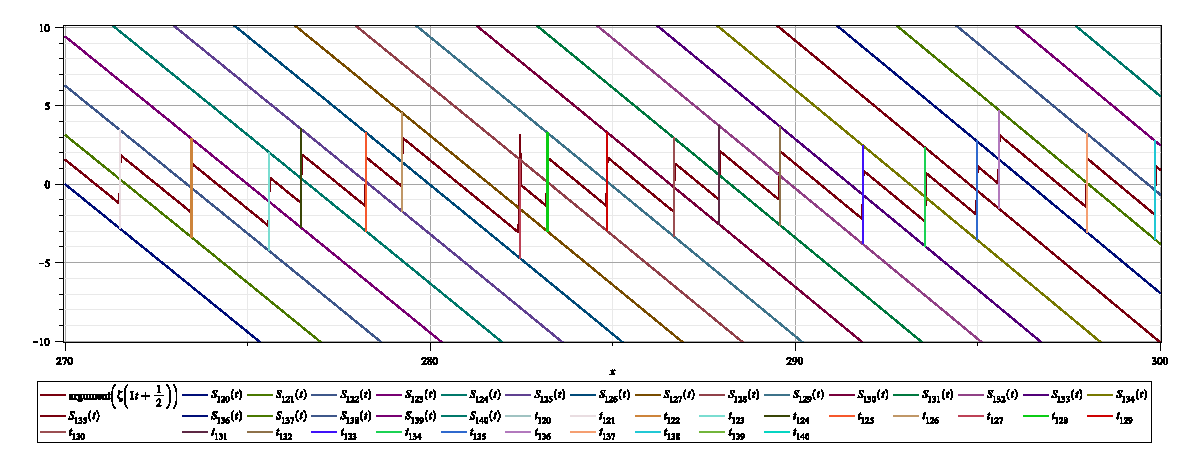
\includegraphics{liftedTwistedAroundFirstBadGramPoints.eps}}
  \caption{$S_n (t)$ and the imaginary parts of the roots of $\zeta \left(
  \frac{1}{2} + i t_n \right)$ marked with verticle lines just touching its
  touching its corresponding pair of neighboring curves $S_n (t)$ for $n = 120
  \ldots 140$ which includes two ``bad'' Gram points at $n = 126$ and $n =
  134$}
\end{figure}

\begin{theorem}
  $\arg \left( \zeta \left( \frac{1}{2} + i g (n) \right) \right) = 0 \forall
  n \in \mathbbm{Z}^+$
\end{theorem}

\begin{proof}
  The argument of any positive number $x$ with $\tmop{Im} (x) = 0$ is equal to
  $0$ and $\tmop{Im} \left( \zeta \left( \frac{1}{2} + i g (n) \right) \right)
  = 0$ since by definition the Gram points are the points where the imaginary
  part of $\zeta$ on the critical line vanishes.
\end{proof}

\begin{conjecture}
  $\tmop{frac} \left( \frac{\vartheta (t)}{\pi} \right) + S (t) \in \{ - 1, 0,
  1 \} \forall 0 < t \in \mathbbm{R}$
\end{conjecture}

\begin{figure}[h]
  \resizebox{5.5in}{3.5in}{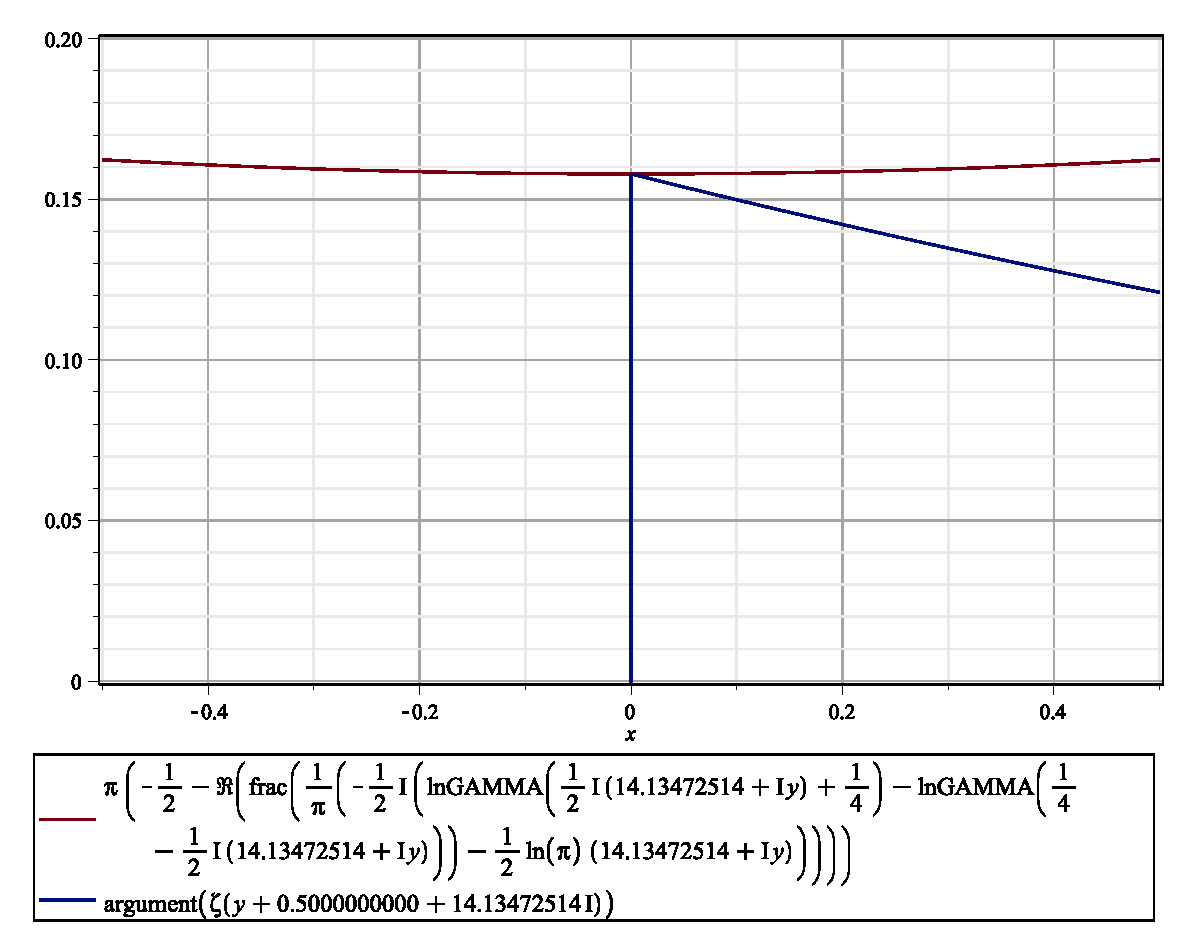
\includegraphics{meet1.eps}}
  \caption{Illustration of convergence around the first zero}
\end{figure}

\subsection{An Equivalent Expression for $S (t)$}

Let
\begin{equation}
  B (t) = N (t) + 2 = \frac{\vartheta (t)}{\pi} + S (t) + 3
\end{equation}
which is Backlund's $\zeta$ zero counting function on the critical strip, plus
$2$, which is valid without assuming the Riemann hypothesis.

\begin{theorem}
  An equivalent expression for $S (t) \forall 0 < t \in \mathbbm{R}$ is
  \begin{equation}
    \begin{array}{cl}
      \mathcal{S} (t) & = S_{B (t)} (t) - \frac{3}{2}\\
      & = B (t) - \frac{3}{2} - \frac{\vartheta (t)}{\pi} - \frac{3}{2}\\
      & = \frac{\vartheta (t)}{\pi} + S (t) + 3 - \frac{3}{2} -
      \frac{\vartheta (t)}{\pi} - \frac{3}{2}\\
      & = \frac{\vartheta (t)}{\pi} + S (t) + 3 - 3 - \frac{\vartheta
      (t)}{\pi}\\
      & = \frac{\vartheta (t)}{\pi} + S (t) - \frac{\vartheta (t)}{\pi}\\
      & = S (t)
    \end{array}
  \end{equation}
\end{theorem}

\begin{proof}
  Since $S (t)$ appears on the left side and right sides of the equation, if
  we subtract $S (t)$ from both sides we get
  \begin{equation}
    \begin{array}{ll}
      0 & = \frac{\vartheta (t)}{\pi} + 3 - \frac{3}{2} - \frac{\vartheta
      (t)}{\pi} - \frac{3}{2}\\
      & = 3 - \frac{3}{2} - \frac{3}{2}\\
      & = 3 - 3\\
      & = 0
    \end{array}
  \end{equation}
\end{proof}

\section{Appendix}

\subsection{Transcendental Equations Satisifed By The Nontrivial Riemann
Zeros}

\begin{definition}
  The \tmverbatim{critical line} is the line in the complex plane defined by
  $\tmop{Re} (t) = \frac{1}{2}$.
\end{definition}

\begin{definition}
  The \tmverbatim{critical strip} is the strip in the complex plane defined by
  $0 < \tmop{Re} (t) < 1$.
\end{definition}

\begin{theorem}
  \label{le}If the limit
  \begin{equation}
    \lim_{\delta \rightarrow 0^+} \arg \left( \zeta \left( \frac{1}{2} +
    \delta + i t \right) \right)
  \end{equation}
  is exists and is well-defined $\forall t$ then the left-hand side of
  Equation (\ref{ae}) is well-defined $\forall t$, and due to monotonicity,
  there must be a unique solution for every $n \in \mathbbm{Z}^+$.
  {\cite[II.A]{z0t}} 
\end{theorem}

\begin{conjecture}
  \label{RH}(The Riemann hypothesis) All solutions $t$ of the equation
  \begin{equation}
    \zeta (t) = 0
  \end{equation}
  besides the trivial solutions $t = - 2 n$ with $n \in \mathbbm{Z}^+$ have
  real-part $\frac{1}{2}$, that is, $\tmop{Re} (t) = \frac{1}{2}$ when $\zeta
  (t) = 0$ and $t \neq - 2 n$.
\end{conjecture}

\begin{lemma}
  \label{fl}If the exact Equation (\ref{ee}) has a unique solution for each $n
  \in \mathbbm{Z}^+$ then Conjecture \ref{RH}, the Riemann hypothesis,
  follows.
\end{lemma}

\begin{proof}
  If the exact equation has a unique solution for each $n$, then the zeros
  obtained from its solutions on the \tmverbatim{critical line} can be counted
  since they are enumerated by the integer $n$, leading to the counting
  function $N_0 (t)$ in Equation (\ref{N0}). The number of solutions obtained
  on the \tmverbatim{critical line} would saturate the counting function of
  the number of solutions on the \tmverbatim{critical strip} so that $N (t) =
  N_0 (t)$ and thus all of the non-trivial zeros of $\zeta$ would be
  enumerated in this manner. If there are zeros off of the critical line, or
  zeros with multiplicity $m \geqslant 2$, then the exact Equation (\ref{ee})
  would fail to capture all the zeros on the critical strip which would mean
  $N_0 (t) < N (t)$. \ {\cite[IX]{z0t}}
\end{proof}

\

\begin{thebibliography}{1}
  \bibitem[1]{z0t}Guilherme Fran{\c c}a  and  Andr{\'e} LeClair.{\newblock}
  Transcendental equations satisfied by the individual zeros of riemann zeta,
  dirichlet and modular l-functions.{\newblock} \tmtextit{Communications in
  Number Theory and Physics}, 2015.{\newblock}
\end{thebibliography}

\end{document}
